\section{Topology Skeletons}
Even though many algorithms can be expressed by parallel maps, some problems require more sophisticated skeletons. The Eden library leverages this problem and already comes with more predefined skeletons, among them the \code{pipe}, \code{ring} and a \code{torus} implementation \cite{eden_cefp, eden_skel_topology}. These seem like reasonable candidates to be ported to our arrow based parallel Haskell to prove that we can express such skeletons with Arrows as well.

\subsection{pipe}

\begin{lstlisting}[frame=htrbl]
pipe :: (ArrowLoop arr, ArrowApply arr,
	ArrowParallel arr (fut a) (fut a) conf, Future fut a) =>
	conf -> [arr a a] -> arr a a
pipe conf fs = unliftFut $ pipeFut conf fs

pipeFut :: (ArrowLoop arr, ArrowApply arr,
	ArrowParallel arr (fut a) (fut a) conf, Future fut a) =>
	conf -> [arr a a] -> arr (fut a) (fut a)
pipeFut conf fs =
	resolve (arr $ \(a, outs) -> lazy $ a : outs) (parEvalNFut conf fs) >>>
	arr last
    where
        resolve :: (ArrowApply arr, ArrowLoop arr) =>
					arr (a, b) c -> arr c b -> arr a b
        resolve transform f =
					loop $ (arr $ \(a, b) -> (b, (f, (transform, (a, b))))) >>>
					second (second app >>> app)
\end{lstlisting}

\subsection{ring}

\begin{lstlisting}[frame=htrbl]
ring :: (ArrowLoop arr, ArrowApply arr, Future fut r, 
ArrowParallel arr (i, fut r) (o, fut r) conf) =>
	conf ->
	arr (i, r) (o, r) ->
	arr [i] [o]
ring conf f = loop $ second (arr rightRotate >>> arr lazy) >>>
	(arr $ uncurry zip) >>> (parMap conf (toFut $ f)) >>> arr unzip

-- similar to Eden's toRD
toFut :: (Arrow arr, Future fut r) =>
	arr (i, r) (o, r) ->
	arr (i, fut r) (o, fut r)
toFut f = (second $ arr get) >>> f >>> (second $ arr put)

-- from Eden:
rightRotate    :: [a] -> [a]
rightRotate [] =  []
rightRotate xs =  last xs : init xs
\end{lstlisting}

\subsection{torus}

\begin{lstlisting}[frame=htrbl]
torus :: (ArrowLoop arr, ArrowChoice arr, ArrowApply arr,
    ArrowParallel arr (c, fut [a], fut [b]) (d, fut [a], fut [b]) conf,
    ArrowParallel arr [(c, fut [a], fut [b])] [(d, fut [a], fut [b])] conf,
    Future fut [a], Future fut [b]) =>
	conf ->
	arr (c, [a], [b]) (d, [a], [b])	->
	arr [[c]] [[d]]
torus conf f =
	loop $ second (arr (map rightRotate) *** arr rightRotate) >>>
	arr (\ (inss, (inssA, inssB)) ->
		zipWith3 lazyzip3 inss (lazy inssA) (lazy inssB)) >>>
	parEvalNM conf (repeat (repeat (ptorus f))) >>>
	arr (map unzip3) >>> arr unzip3 >>> threetotwo

lazyzip3 :: [a] -> [b] -> [c] -> [(a, b, c)]
lazyzip3 as bs cs = zip3 as (lazy bs) (lazy cs)

ptorus :: (Arrow arr, Future fut [a], Future fut [b]) =>
          arr (c, [a], [b]) (d, [a], [b]) ->
          arr (c, fut [a], fut [b]) (d, fut [a], fut [b])
ptorus f =
	arr (\ ~(c, fas, fbs) -> (c, get fas, get fbs)) >>>
	f >>>
	arr (\ ~(c, as, bs) -> (c, put as, put bs))

threetotwo :: (Arrow arr) => arr (a, b, c) (a, (b, c))
threetotwo = arr $ \ ~(a, b, c) -> (a, (b, c))

parEvalNM :: (ArrowChoice arr, ArrowApply arr, ArrowParallel arr a b conf,
	ArrowParallel arr [a] [b] conf) =>
	conf -> [[arr a b]] -> arr [[a]] [[b]]
parEvalNM conf = listApp . (map (parEvalN conf))
\end{lstlisting}

\begin{figure}[ht]
	\centering
	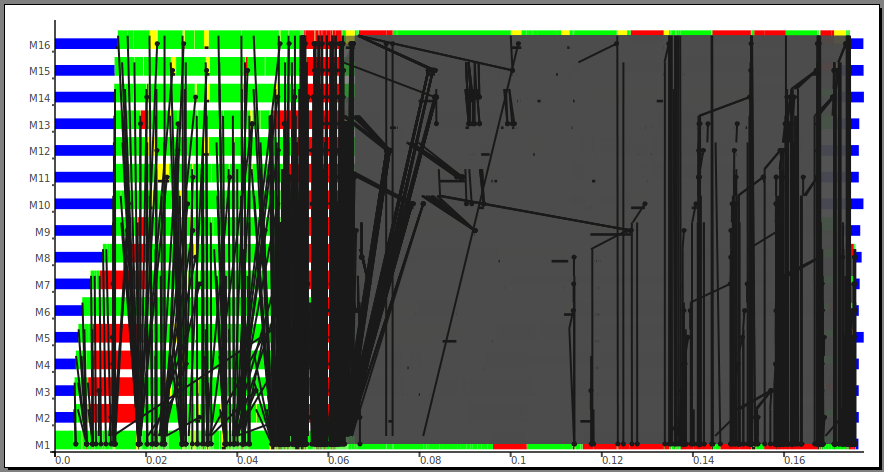
\includegraphics[width=0.9\textwidth]{images/torus_matrix_parrows}
	\caption[without Futures]{Matrix Multiplication with a torus (Parrows)}
\end{figure}

\begin{figure}[ht]
	\centering
	\includegraphics[width=0.9\textwidth]{images/torus_matrix_eden}
	\caption[with Futures]{Matrix Multiplication with a torus (Eden)}
\end{figure}